\section{Dynamic Visual Querying}\label{sec:visualQuery}
To facilitate astronomers' easy discovery of time intervals similar to a ROI/SOI (\textbf{G3}) or those validating specific hypotheses (\textbf{G4}), 
TimeTubesX provides two different user-initiative visual query interfaces: query-by-example (QBE) and query-by-sketch (QBS).
Both are designed to help users identify interesting similar patterns (\textbf{T4}), and our matching algorithm allows for a fuzzy search (\textbf{T5}).
% those more subtle than the well-known patterns described in \autoref{sec:automaticExtraction}.

\subsection{Query-by-Example}\label{sec:QBE}
% background and overview
While the TimeTubes view helps users analyze time variation patterns,
it still remains challenging for users to build queries for multi-dimensional, time-dependent data.
Our QBE interface allows users to specify an interesting behavior as a ROI with simple interactions through the TimeTubes or scatterplots views.
Users can not only pick a part of time-series data as an input for a query but also flexibly select specific variables that should be used in the query to reflect their intentions. 
This allows users to easily and intuitively search long-term datasets for interesting patterns with minimal required user inputs.

Fig.~\ref{fig:querySpecificationPanel} (B) shows our QBE interface.
% First, users specify the time interval by either clicking on the corresponding slice in the 3D Timetubes view, or by defining a region in the scatterplot view (see \autoref{fig:querySpecificationPanel} (B)(1)).
To facilitate visual verification by users, a time interval selected through the TimeTubes or scatterplots views in (2, red highlight) is automatically extracted and displayed in the query panel (1).
% The selected time interval is highlighted in red in both views.
% Our system automatically extracts the selected time interval and displays it in the query panel (2) to facilitate visual verification by users.
After selecting the initial time interval, users can then fine-tune and adjust their query by selecting the variables that should be queried on. 
This is crucial for effective support of queries on multi-dimensional data.
Based on the selected variables, 
our system interactively updates the appearance of the 3D tube for the selected time interval in (1), visually encoding only currently selected variables.
For example, when users remove the variable $C$ from the query, the tube loses color variation and becomes a gray tube, as shown in (1).
% % high-level overview
% Our QBE interface was designed for time-dependent multi-dimensional data. 
% Users first pick the part of the dataset that should serve as input for a query. In a second step, however, they are also able to select the specific variables and the exact time span that should be used in the query, which is dynamically updated in the query panel (see \autoref{fig:querySpecificationPanel} (B)).
% This makes it easier for users to fine-tune and adjust queries for highly complex datasets.
% %
% %\autoref{fig:querySpecificationPanel} (B) shows our QBE panel.
% % THIS IS JUST UI
% We allow users to select a ROI for their query directly in the TimeTubes or scatterplot views.
% First, users specify the time interval by either clicking on the corresponding slice in the 3D Timetubes view, or by defining a region in the scatterplot view (see \autoref{fig:querySpecificationPanel} (B)(1)).
% %a part of the 3D tube or setting a region on scatterplots view, as shown in part (1). 
% The selected time interval is highlighted in red in both views. % of TimeTubes and scatterplots.
% %
% % THIS IS MUCH MORE INTERESTING - highlight WHY you are doing this (multi-dim queries, visually define those, give immediate user feedback)
% Our system automatically extracts the selected time interval and displays it in the query panel (2) to facilitate visual verification by the user.
% %as another 3D tube for the users to easily validate what they selected in part (2).
% After selecting the initial time interval, users can then fine-tune their query by selecting the variables that should be included in the query. This is crucial to support queries on multi-dimensional data.
% Based on the selected variables, 
% our system interactively updates the appearance of the 3D tube for the selected time interval, to only visually encode the currently selected variables.
% For example, when the users removes $C$ from the query, the tube loses color variation and becomes a gray tube, as shown in part (2).
After defining the query, users can adjust main parameters (i.e., normalization and polar coordinates options) for our matching algorithm (see Section~\ref{sec:matchingAlgorithm}). 
%We explain the matching algorithm between the query and time intervals in \autoref{sec:matchingAlgorithm}.
%
% Both options enable a fuzzy pattern search.
% %The Normalization option and polar coordinates option realize fuzzy pattern search.
% The normalization option triggers that the system normalizes the query and time intervals into the range of $[0, 1]$.
% Subsequently, the pattern search places great significance on the \emph{shape} of the time variations whereas the actual length of the time interval will be ignored.
% With the polar coordinates option, 
% $q(t)$ and $u(t)$ are converted into polar coordinates ($r-\theta$ domain) before computing similarities.
% Subsequently, the pattern search will also extract patterns that rotating around the origin of the Stoke plane.

\begin{figure}[tb]
    \centering
    \begin{minipage}{0.24\linewidth}
        \centering
        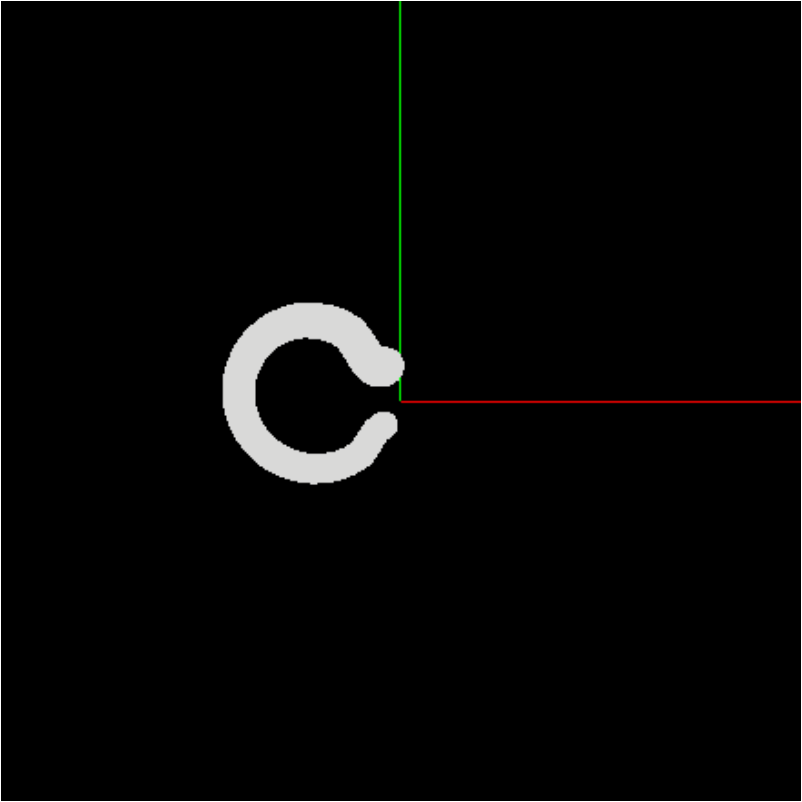
\includegraphics[width=.99\linewidth]{vgtc_journal_latex/figures/QBE.png}
        \footnotesize{\sf (a)~Query.}
    \end{minipage}
    \begin{minipage}{0.75\linewidth}
        \centering
        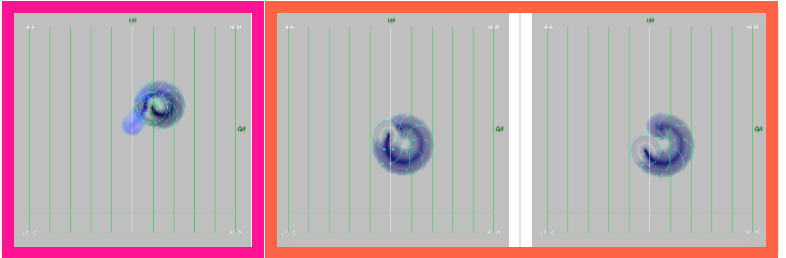
\includegraphics[width=.99\linewidth]{vgtc_journal_latex/figures/QBEdemodataResults_revised.png}
        \footnotesize{\sf(b)~Results for the query in (a).}
    \end{minipage}
    \caption{QBE for our synthetic dataset in Fig.~\ref{fig:synthesisData}. 
        We pick the time interval with a small circular pattern (the leftmost red pattern in Fig.~\ref{fig:synthesisData}~(b)) for a query in (a). 
        Our method exactly extracted other time intervals with small circular patterns (the two red patterns from the right in Fig.~\ref{fig:synthesisData}~(b)).
        The outline color corresponds to the color in Fig.~\ref{fig:synthesisData}~(b).}
    \label{fig:QBEDemodata}
\end{figure}
\textsf{Experimental results.\ } We verified the effectiveness of our QBE method with our synthetic data.
The red circular patterns in Fig.~\ref{fig:synthesisData}~(b) have a similar shape but different time lengths, scales, or locations in the Stokes plane.
We used the leftmost red time interval in (b) as an input query, as shown in Fig.~\ref{fig:QBEDemodata}~(a).
We selected $q$ and $u$ as active variables and used the normalization and polar coordinates options to detect time intervals with different scales or different positions.
The length of the target time interval was set to 5 to 20 days.
% Due to the small size of the synthetic dataset, we set the sliding window step size to 2. 
We used $\rm{DTW}_{\rm D}$ as a distance function.
Note that we detail the options and parameters related to the matching process in Section~\ref{sec:matchingAlgorithm}.
Fig.~\ref{fig:QBEDemodata}~(b) shows the top three results of our QBE query.
The color of the rectangles corresponds to those used in Fig.~\ref{fig:synthesisData}~(b).
We were able to detect all time intervals with a similar shape in our synthetic dataset.
%The time intervals with a similar shape were definitely detected by the proposed QBE.
Note that the time interval specified for the query itself is omitted from the results.

\subsection{Query-by-Sketch}\label{sec:QBS}
% background and overview
TimeTubesX also allows users to query their data by manually drawing time variation patterns onto a 2D sketch interface.
Our QBS interface provides an intuitive and accessible way for users to specify patterns for complex multi-dimensional, semi-structured, time-dependent blazar datasets and to test their high-level hypotheses.
% To allow users to easily draw a pattern for multi-dimensional, semi-structured, time-dependent blazar datasets on a 2D sketch pad and test their abstract hypotheses of blazar behaviors, 
% we provide a novel QBS interface.
Rouxel et al.~\cite{Rouxel2014} state that an input trajectory by analog gestures are characterized by three dimensions: space, time, and force.
% To limit the complexity for users, our interface detects three input parameters: $x$ position, $y$ position, and either speed \emph{or} force.
To maintain the intuitiveness, 
we use space to determine the $x$ and $y$ positions of the stroke
and use either drawing speed or drawing pressure to define the stroke width 
so that users can describe time variations of multiple dimensions simultaneously.
Using the drawing speed option, the longer a cursor stays on a single point, the wider the curve at the point becomes.
To take into account other variables that are not described in sketching gestures, 
our QBS interface allows users to assign filtering constraints for each variable.
Thus, a sketch-based query for multi-dimensional, semi-structured, time-dependent data can be built with a single gesture
without sketching time variation patterns several times.

% ui and interactions
Fig.~\ref{fig:querySpecificationPanel} (C) shows the QBS query specification panel.
First, users define which variables are assigned to the $x$ and $y$ axes of the sketch pad and the stroke width (see panel (5)).
Second, they sketch a time variation pattern on a 2D sketch pad UI (3),
where the stroke is shown in black and its width is shown in blue.
% After drawing, our system automatically converts the sketch into a Cubic Bezier curve and beautifies the input stroke to remove undesired artifacts due to shaky input. 
After drawing, our system automatically beautifies the input stroke by fitting it to a cubic Bezier curve with as few segments as possible with ‘simplify’ method from Paper.js~\cite{paper_framework}.
After their initial drawing, users can further adjust the sketch
by adding, removing, or moving control points, or by changing the stroke width.
Furthermore, users are allowed to assign filtering constraints to each of the control points on the input sketch, as shown in part (4).
% By clicking on a control point, a popup panel appears next to the selected point, as shown in part (4).
Users can define value ranges for each variable at the control point, which will be subsequently used when evaluating the query.

% Our QBS interface realizes a fuzzy pattern search based on hand-drawn user input to flexibly find interesting time intervals or test new hypotheses.
% TODO: Missing general intro that we use a 2D panel and can use speed, pressure for additional parameters, to intuitively and quickly sketch queries. represented as curves/splines. 

% % 
% \autoref{fig:querySpecificationPanel} (C) shows the QBS query specification panel.
% First, users define which variables are assigned to the $x$ and $y$ axes of the sketch pad and the width of the stroke (see panel (3)).
% TimeTubesX provides a 2D sketch pad UI (1), where the stroke is shown in black and its width is shown in blue. 
% According to Rouxel et al.~\cite{Rouxel2014}, there are three dimensions used to characterize a trajectory when sketching: space, time, and force. 
% To limit the complexity for the user, we limit our input to three parameters: $x$ position, $y$ position, and either time \emph{or} force.
% In particular, we use space for expressing two variables ($x$ and $y$ axes),
% and use either drawing speed or drawing pressure to define the width of the stroke.
% %so that either time or force can be used to express another variable.
% %Our sketch pad converts either drawing speed or drawing pressure into the width of the stroke.
% Using the drawing speed option, the longer a cursor stays on a single point, the wider the curve at this point becomes. %width of the part gets larger. 
% After drawing, our system automatically converts the sketch into a curve, and smooths the input stroke to remove undesired artifacts due to shaky input. 
% %Therefore, the users do not need to care about the shakes of hands.
% After their initial drawing, users can further adjust the sketch
% by adding, removing, or moving control points, or changing the width of the stroke. % with simple and intuitive interactions.
% %\autoref{fig:querySpecificationPanel} (C) show
% % unnecessary The query modification menus are shown as icons in the upper part of part (1).
% Furthermore, users can assign filtering constraints to each of the control points on the input sketch.
% By clicking on a control point, a popup panel appears next to the selected point, as shown in part (2).
% Users can define value ranges for each variable at the control point, which will be subsequently used when evaluating the query.% and then the corresponding label showing the variable names appears above the control point.
% %According to the assigned filtering constraints, TimeTubesX filters the extraction results.
% %In part (3), they choose which variable to assign to the stroke width, the length of the input sketch, and so on.
% %In QBS, they can set the parameters for matching as well.

% Furthermore, TimeTubesX allows users to easily re-use and share interesting queries by exporting and importing a query as a JSON file.
% Furthermore, TimeTubesX allows users to export and import a query as a JSON file for easy reuse and sharing.
% TimeTubesX supports export and import of queries as a JSON file.
%Re-utilizing frequently used queries makes the analysis more efficient, 
% This allows users to share interesting queries with others, and also allows users to easily re-use frequently used queries.
%It is also helpful for them to review their input.

\begin{figure}[tb]
    \centering
    \begin{minipage}{0.49\linewidth}
        \centering
        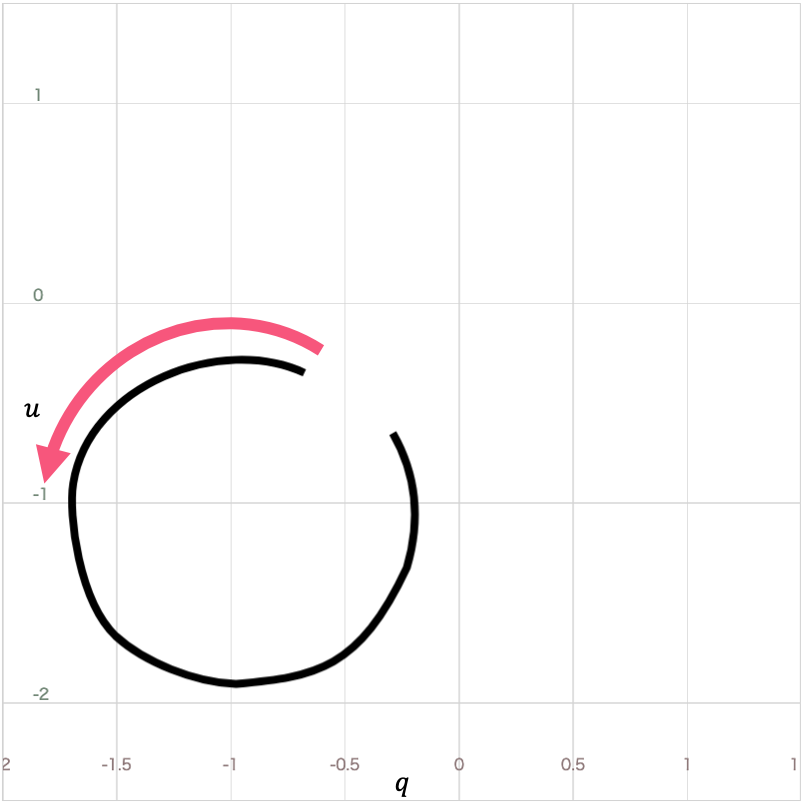
\includegraphics[width=.9\linewidth]{vgtc_journal_latex/figures/QBSSketchwithoutWidth.png}
    \end{minipage}
    \begin{minipage}{0.49\linewidth}
        \centering
        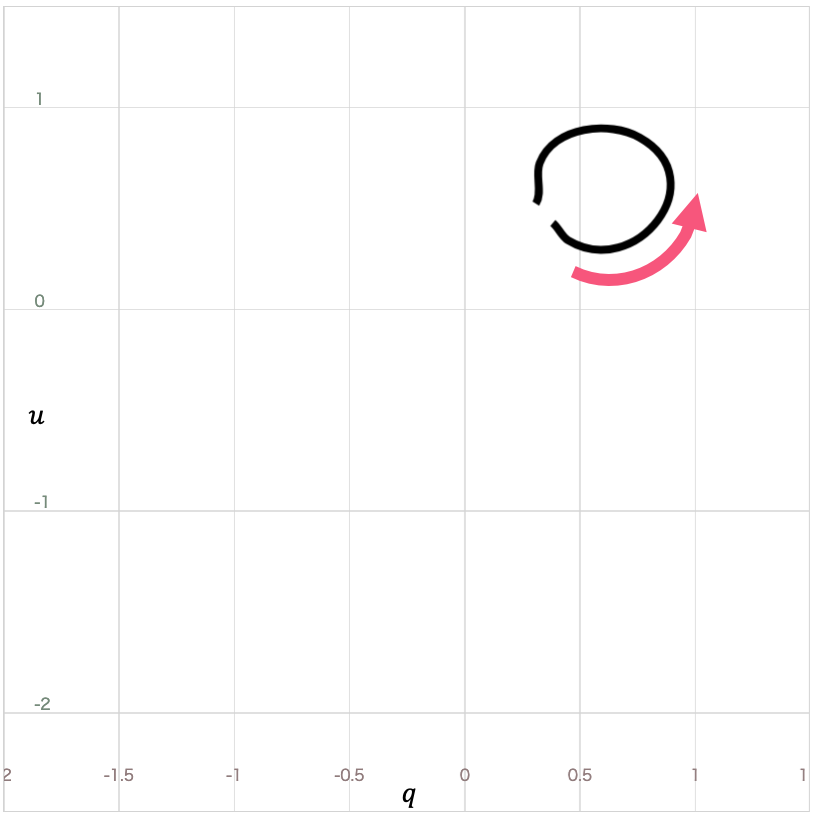
\includegraphics[width=.9\linewidth]{vgtc_journal_latex/figures/QBSResultQuerywithoutWidth.png}
    \end{minipage}
    \begin{minipage}{0.49\linewidth}
        \centering
        \footnotesize{\sf (a)~Hand-drawn sketch query for a small circular pattern.}
    \end{minipage}
    \begin{minipage}{0.49\linewidth}
        \centering
        \footnotesize{\sf (b)~A sketch based on the upper left result in (c). 
        % to extract similar patterns, as shown in (d).
        }
    \end{minipage}
    \begin{minipage}{0.49\linewidth}
        \centering
        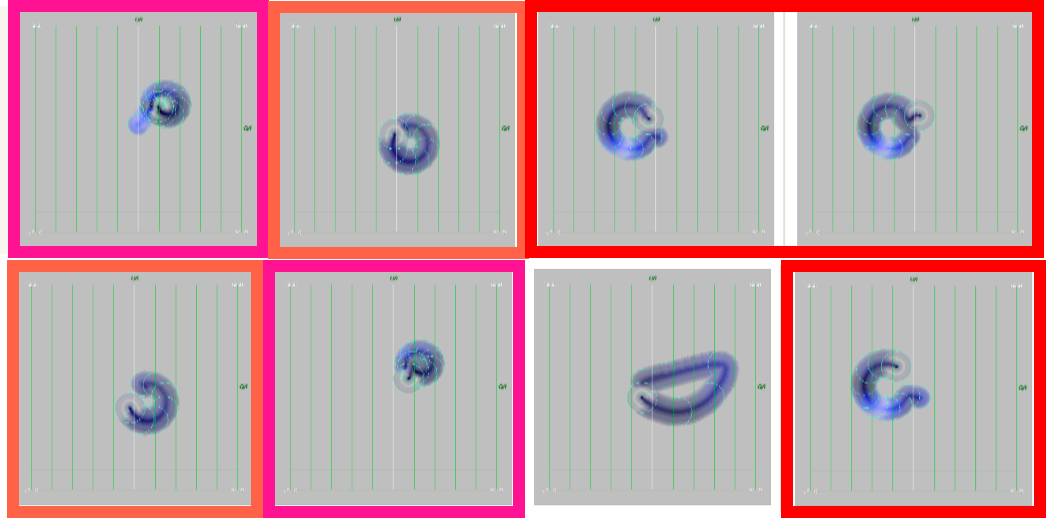
\includegraphics[width=.99\linewidth]{vgtc_journal_latex/figures/QBSResultsHanddrawn_revised.png}\\
        \footnotesize{\sf (c)~Results for the query in (a).}
    \end{minipage}
    \begin{minipage}{0.49\linewidth}
        \centering
        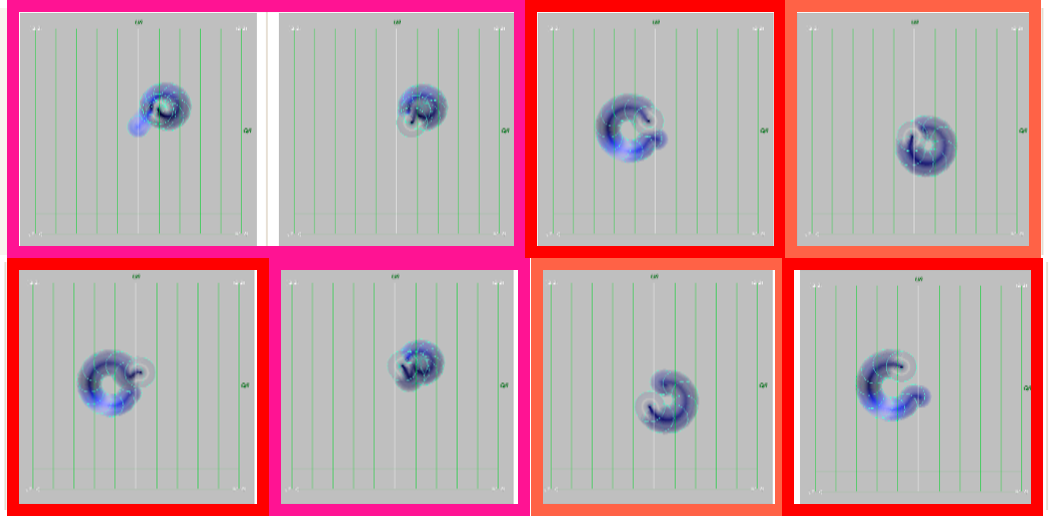
\includegraphics[width=.99\linewidth]{vgtc_journal_latex/figures/QBSResultsResultQuery_revised.png}\\
        \footnotesize{\sf (d)~Results for the query in (b).}
    \end{minipage}
    \caption{QBS results for our synthetic dataset in Fig.~\ref{fig:synthesisData}.
        %The outline color corresponds to the color in \autoref{fig:synthesisData}~(b).
        With a hand-drawn sketch in (a), an unexpected result is highly ranked (white outline) in (c). 
        With a sketch based on actual data values (b), no unexpected results appear, as illustrated in (d).
        % Upon further refinement of the initial sketch to more closely resemble actual data values (b), no unexpected results appear anymore.
        }
    \label{fig:QBSDemodata}
\end{figure}
%
\textsf{Experimental results.\ } We demonstrated the effectiveness of our QBS interface with our synthetic dataset.
%To demonstrate the effectiveness of our QBS interface,
%we have applied QBS to the synthesis data.
%To find out the time intervals with a small circular pattern,
First, we made a query with the sketch shown in Fig.~\ref{fig:QBSDemodata}~(a) to extract time intervals with small circular patterns. 
The sketch pad plane corresponds to the Stokes plane and, for simplicity, the stroke width is not used.
To detect time intervals with a similar shape but different positions or scales, we used the normalization and polar coordinates option.
% Due to the small size of the synthetic dataset, we set the sliding window step size to 2.
Fig.~\ref{fig:QBSDemodata}~(c) shows the top eight results of our QBS method for the query in (a).
The outline color of each thumbnail image matches the color of the corresponding circular pattern in Fig.~\ref{fig:synthesisData}~(b).
% We enclose the results that include the small circular pattern in rectangles 
% The outline color of the individual results corresponds to the colors used in the circular patterns in
% whose color corresponds to the colors used in the circular patterns in \autoref{fig:synthesisData}~(b).
All three time intervals highlighted in red in Fig.~\ref{fig:synthesisData}~(b) were properly extracted.
Nevertheless, an unexpected result (i.e., the thumbnail with no outline color in Fig.~\ref{fig:synthesisData}~(c)) was highly ranked as a candidate similar to the input pattern due to the ambiguities of a hand-drawn sketch.
We address this problem by incorporating fact-guided querying (see Section~\ref{sec:factDrivenQuerying}). 

%
\subsection{Query Matching Algorithm}\label{sec:matchingAlgorithm}
\begin{figure}[tb]
    \begin{minipage}{0.62\linewidth}
        \centering
        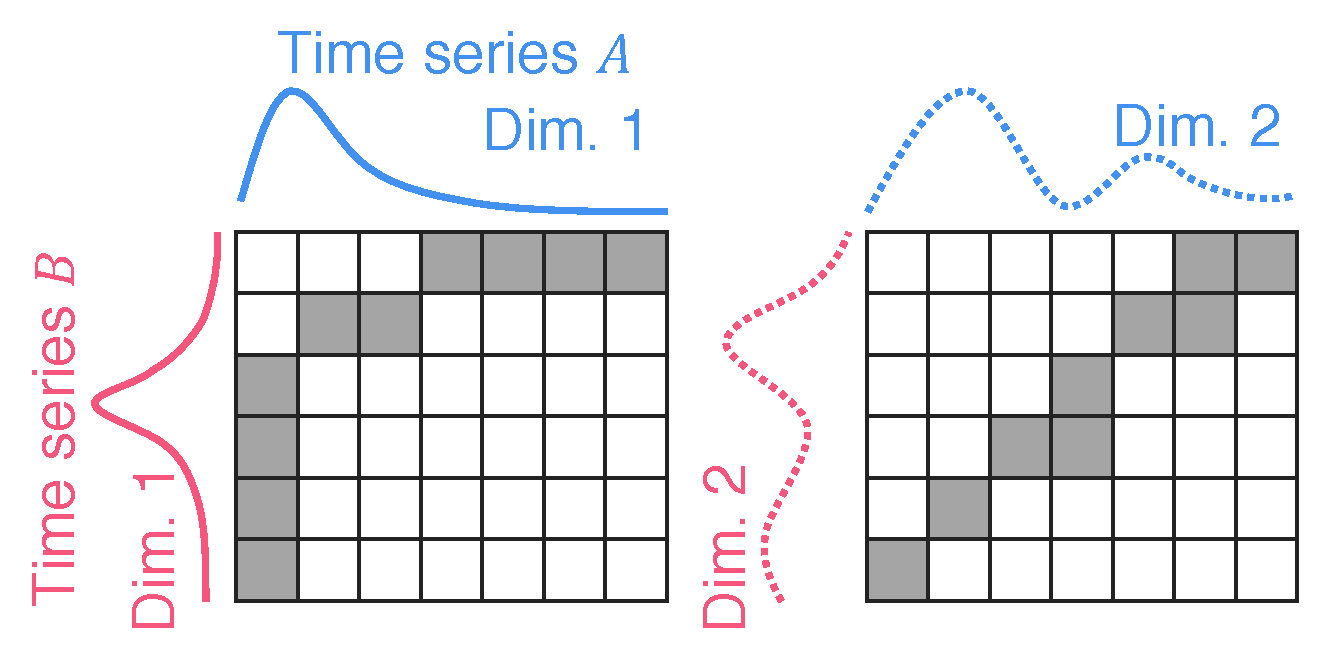
\includegraphics[width=.95\linewidth]{vgtc_journal_latex/figures/DTWI.pdf}\\
    \end{minipage}
    \begin{minipage}{0.37\linewidth}
        \centering
        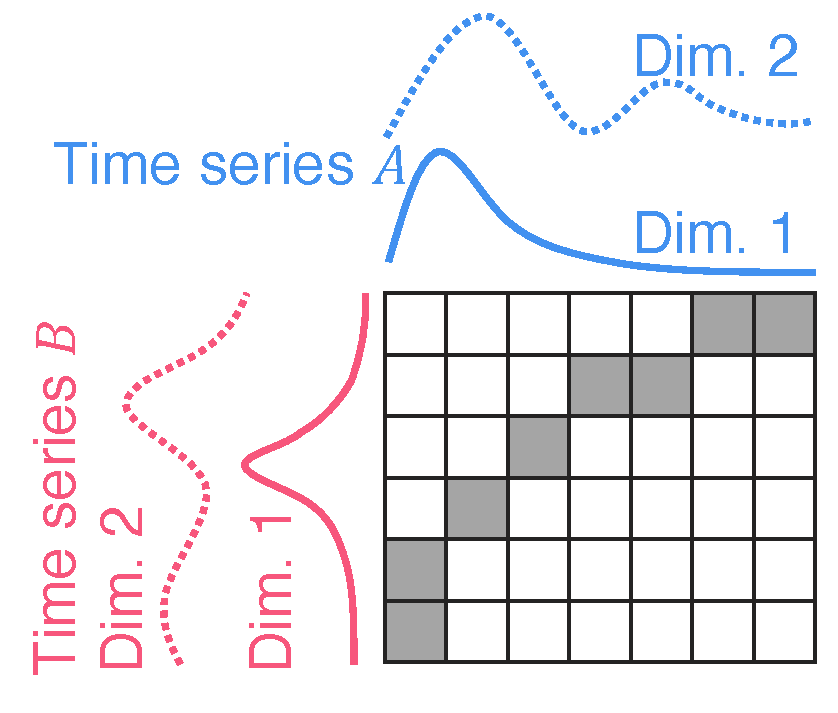
\includegraphics[width=.95\linewidth]{vgtc_journal_latex/figures/DTWD.pdf}\\
    \end{minipage}
    \begin{minipage}{0.62\linewidth}
        \centering
        \footnotesize{\sf(a)~${\rm DTW}_{\rm I}$}
    \end{minipage}
    \begin{minipage}{0.37\linewidth}
        \centering
        \footnotesize{\sf(b)~${\rm DTW}_{\rm D}$}
    \end{minipage}
    \caption{DTW options for dealing with multi-dimensional data.
    ${\rm DTW}_{\rm I}$ warps each dimension independently, whereas all dimensions are warped dependently in ${\rm DTW}_{\rm D}$.}
    \label{fig:DTW}
\end{figure}
%
There are many different methods to compute the distance between two time series, such as the Euclidean distance, uniform scaling, or dynamic time warping (DTW)~\cite{Berndt1994}.
TimeTubesX uses DTW
because it aligns two time series elastically and thus supports the comparison of time series with different lengths.
Additionally, it can compute the distance between two time series that are similar, but locally out of phase.
%more intuitively even if they are out of phase in the time direction. 
According to Eichmann and Zgraggen~\cite{Eichmann2015}, the DTW similarity measurement seems to most closely match human perception.
There are multiple solutions for dealing with multi-dimensional data in DTW. 
TimeTubesX implements two options, ${\rm DTW}_{\rm I}$ (independent) and ${\rm DTW}_{\rm D}$ (dependent), both based on the work of Shokoohi-Yekta et al.~\cite{Shokoohi-Yekta2015}.
%${\rm DTW}_{\rm Independent}$ (${\rm DTW}_{\rm I}$) and ${\rm DTW}_{\rm Dependent}$ (${\rm DTW}_{\rm D}$). 
%The ideas come from Shokoohi-Yekta et al.~\cite{Shokoohi-Yekta2015}.

${\rm DTW}_{\rm I}$ computes the distance between two time series for each dimension of the data separately (see Fig.~\ref{fig:DTW}~(a)). In the final step, it adds up all those individual distances to the final distance measure.
%${\rm DTW}_{\rm I}$ makes each dimension of time series warp irrespective of other dimensions and then cumulates the distances of all dimensions, as illustrated in \autoref{fig:DTW}~(a).
% ${\rm DTW}_{\rm I}$ defines the distance between two time series as a cumulative distance of all dimensions in the time series.
% In other words, it makes each dimension warp irrespective of other dimensions, as illustrated in \autoref{fig:DTW}~(a).
Consequently, this approach focuses more on the similarity of each dimension and less on correlations between different dimensions.
%Consequently, this takes more account not of correlations among dimensions but of similarity of each dimension.
% Consequently, ${\rm DTW}_{\rm I}$ regards time intervals each of whose dimensions has a similar time variation pattern to the input pattern as 
% Consequently, the time variation of each dimension looks similar, 
% but correlations among dimensions may decrease.
% wrong: first accumulates the signal from all dimensions for each time series individually, and then computes the distance between those two accumulated time series (see \autoref{fig:DTW}~(b)).
${\rm DTW}_{\rm D}$, on the other hand, computes the distance between two data samples directly over all dimensions (i.e., as Euclidean distance in $n$-dimensional space), as seen in Fig.~\ref{fig:DTW}~(b).
Therefore, this method focuses more on correlations among the different dimensions of a time series and less on the similarities of individual dimensions. 
%takes more account of correlations among dimensions than similarity of each dimension.
By default, our system uses ${\rm DTW}_{\rm D}$ because correlations among variables are significantly more important for blazar behavior analysis.

We use a sliding window approach in our matching algorithm.
%, the interactive feature extraction picks up a time interval from long-term data 
%and then computes the distance between the input query and the time interval according to the selected option.  
Users can set the window size and the step size of the sliding window and also set a constraint on the largest allowed temporal shift (i.e., warping window size)
% The warping window size determines the largest allowed temporal shift 
in the process of finding the best alignment between the query and time series.
Users can specify these parameters at the bottom of the query specification panel in Fig.~\ref{fig:UIFeatureExtraction}~(A).
Note that multiple time intervals with different lengths but including the same time points can be presented in the extraction results (see Fig.~\ref{fig:QBEDemodata} and Fig.~\ref{fig:QBSDemodata}~(c) and (d)). %because of the use of a sliding window approach.
The timelines in Fig.~\ref{fig:UIFeatureExtraction}~(C) help users recognize such time intervals. 
% Users can identify the groups of the extraction result by giving a glance at the timeline.

Normalization and polar coordinates options enable a fuzzy pattern search.
%The Normalization option and polar coordinates option realize fuzzy pattern search.
The normalization option triggers the system to normalize a query and time intervals into the range of $[0, 1]$.
Subsequently, the pattern search places great significance on the \emph{shape} of the time variations, whereas the actual value ranges will be ignored.
With the polar coordinates option, 
$q(t)$ and $u(t)$ are converted into polar coordinates ($r-\theta$ domain) before computing similarities.
Subsequently, the pattern search with the normalization and polar coordinates options will also be able to extract patterns rotating around the origin of the Stoke plane.

%
%
\subsection{Fact-Guided Querying}\label{sec:factDrivenQuerying}
To support quick and iterative query refinement, TimeTubesX allows users to re-utilize individual extraction results as an input for follow-up queries, a process we termed \emph{fact-guided querying}.
% We call this \emph{fact-driven querying},  
% since it allows users to easily search for time intervals similar to actual data measurements, implying that it makes it easy for users to find common features.
By iteratively updating a query, users can, in a step-by-step manner, identify more observable time intervals that reflect their intentions.
% In other words, the feature extraction and visual query interface realizes a self-organizing query refinement.
% With a refined query, users can find more observable time intervals which reflect their intentions more. 
Therefore, fact-guided querying contributes immensely to drilling-down into data as a part of the visual exploration framework of TimeTubesX in Fig.~\ref{fig:framework}.
In QBE, users can switch variables used in the matching process and modify the time range of the query, while in QBS, users can adjust the scale, shape, and axis of the input query or add further filtering constraints.
% initial interesting time intervalを見つける手間を省いたり?ユーザの意図をより反映したtime intervalに基づいてクエリを作成したり?白紙からスケッチを書かないで、実際の値に基づいて任意のスケッチを作成したりできる
Thus, it helps users perform further pattern searches based on the interesting time interval found in the previous process or create a sketch-based query from references to actual data measurements instead of from a blank sketch pad.
% not from a blank sketch pad but with reference to actual data measurements.

Our system allows users to build a fact-guided query with simple interactions, i.e.,
dragging an extraction result either into the QBE interface (part (2) in Fig.~\ref{fig:querySpecificationPanel}~(B)) or into the sketch pad of the QBS interface (part (3) in Fig.~\ref{fig:querySpecificationPanel}~(C)).
%
%Due to the fact-driven querying function, they can 
%In particular, when changing the axis of the sketch pad, 
%the sketch is automatically updated with reference to the selected result.
%The sketch is 2D, but multi-dimensional data is stored internally as a vital part of a query.


\textsf{Experimental results.\ } We illustrated the usefulness of the fact-guided querying approach with our synthetic dataset.
As discussed in Section~\ref{sec:QBS}, 
hand-drawn sketch queries, such as Fig.~\ref{fig:QBSDemodata}~(a), work well for finding time intervals with a specific feature,
but ambiguities of hand-drawn sketches may sometimes lead to unexpected results, as shown in (c).
%
% \autoref{fig:QBSDemodata}~(a) shows an initial hand-drawn query. %and search for time intervals with a similar feature.
If the extraction results for the query in (a) sufficiently represent users' intentions, one of the results can be used as an input to refine results of the next visual query.
%When we find time intervals which sufficiently validate our intention, we can use the one of the results for yet another query of the visual query.
% For the query in (b), 
We chose the top left result of (c) and used it as an input to our QBS method, as shown in (b). 
%and converted it for a query in QBS.
The sketch pad plane in (b) coincides with the Stokes plane.
Thereafter, we ran QBS in the same parameter settings as the example in Section~\ref{sec:QBS}.
As shown in the top eight extraction results in (d),  % of QBS with the query in (b).
this refined query in (b) no longer produces any highly-ranking outliers or unexpected results.
% does not result in highly ranking any outliers or unexpected results any longer.
%As the red rectangles illustrate,
%unexpected results were not highly ranked any longer.
%The application examples in \autoref{fig:QBSDemodata} illustrate that the fact-driven querying effectively works for the query refinement.



% \begin{figure}[tb]
%     \centering
%     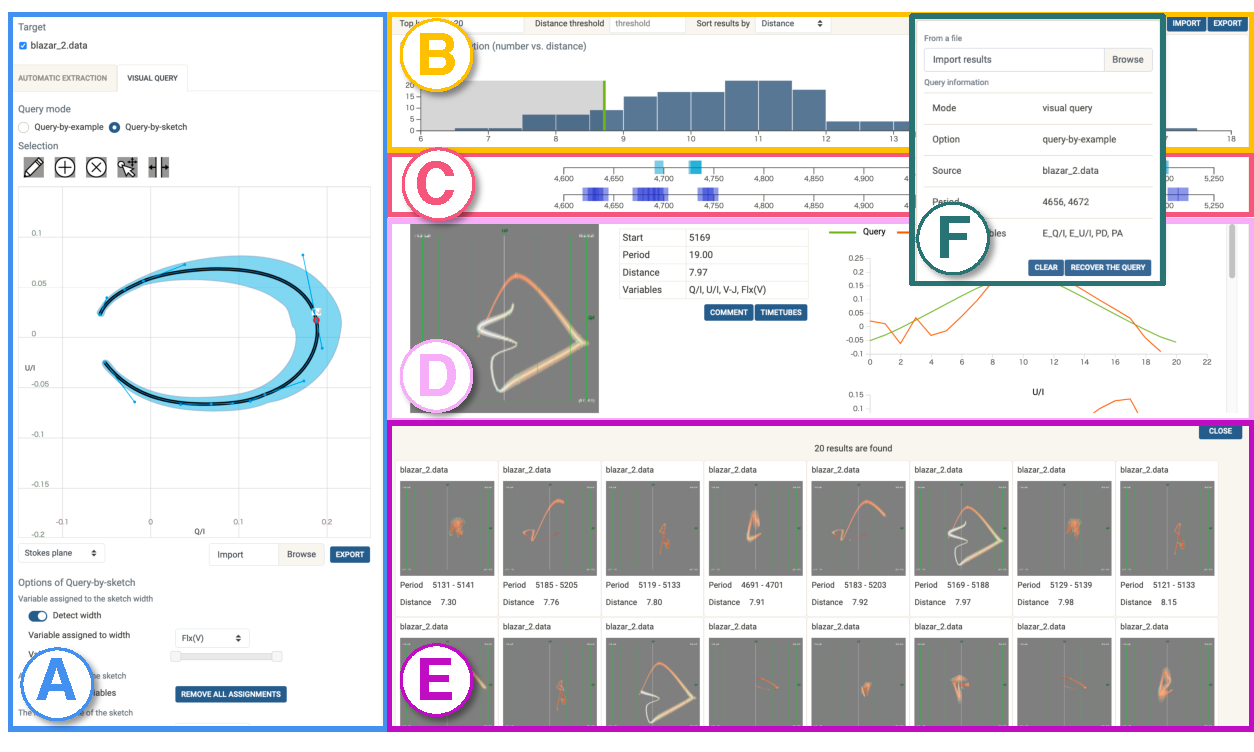
\includegraphics[width=.99\linewidth]{images/GUI.pdf}
%     \caption{User interface of the interactive feature extraction. (a)~Query specification panel; (b)~Parameters for ranking, filtering, and displaying extraction results and a histogram summarizing distance distribution of extraction results; (c)~The timeline overviewing displayed extraction results; (d)~Detail information panel for a selected result; (e)~A collection of thumbnails for extraction results.}
%     \label{fig:UIFeatureExtraction}
% \end{figure}
% \begin{figure}[tb]
%     \centering
%     \begin{minipage}{0.6\linewidth}
%         \centering
%         \includegraphics[width=.99\linewidth]{images/QBEMenuLabel.png}
%     \end{minipage}
%     \begin{minipage}{0.39\linewidth}
%         \centering
%         \includegraphics[width=.97\linewidth]{images/QBSMenuLabel.png}
%     \end{minipage}
%     \begin{minipage}{0.6\linewidth}
%         \centering
%         \footnotesize{\sf (a)~Query-by-example.}% (1)~Panels for specifying ROI from TimeTubes view or scatterplots view; (2)~A 3D tube for selected time interval.}
%     \end{minipage}
%     \begin{minipage}{0.39\linewidth}
%         \centering
%         \footnotesize{\sf (b)~Query-by-sketch.}% (1)~Sketch pad for drawing a query; (2)~A popup panel for filter constraints assignment; (3)~Parameters for controlling the sketch pad and sketch stroke.}
%     \end{minipage}
%     \caption{Query specification panel in the interactive feature extraction (Fig.~\ref{fig:UIFeatureExtraction}~(a)).}
%     \label{fig:QuerySpecification}
% \end{figure}


% Fig.~\ref{fig:UIFeatureExtraction} shows the designate user interface, 
% where QBS option is selected.
% The users are allowed to choose either option of the visual query and specify a query in part (a).
% This query specification panel in part (a) with each option of the visual query is illustrated in Fig.~\ref{fig:QuerySpecification}.
% After running the similarity search, 
% the system displays extraction results according to the parameteres in part (b), 
% such as preferred order of results, threshold for results, and the number of displayed results.
% A histogram summarizing the distance distribution of the extraction results appears in part (b),
% which is helpful for the users to decide how many results to show.
% By adjusting the gray area on the histogram,
% the users can alter the number of the displayed results. 
% The timeline in part (c) overviews the location of the extraction results,
% which enables the users to understand temporal distributions of the results.
% Detail information of the result, such as limit timestamps of the time interval and the distance between the query and time interval, will appear in part (d)
% by selecting a result from the collection of thumbnails in part (e).

% QBE gives a kind of flexibility to a selected example.

% Such flexibility makes it easier for the users to reflect their intentions to the example.

% The task \textbf{T4} is effectively supported by QBE.
% Moreover, \textbf{T5} can also be supported by using a normalization option and polar coordinates option.

% Users can find out time intervals with similar shapes to the query but with different sizes.

% With the combination of both options,
% the users can also find out time intervals at different positions from the query.

    % \begin{minipage}{0.55\linewidth}
    %     \centering
    %     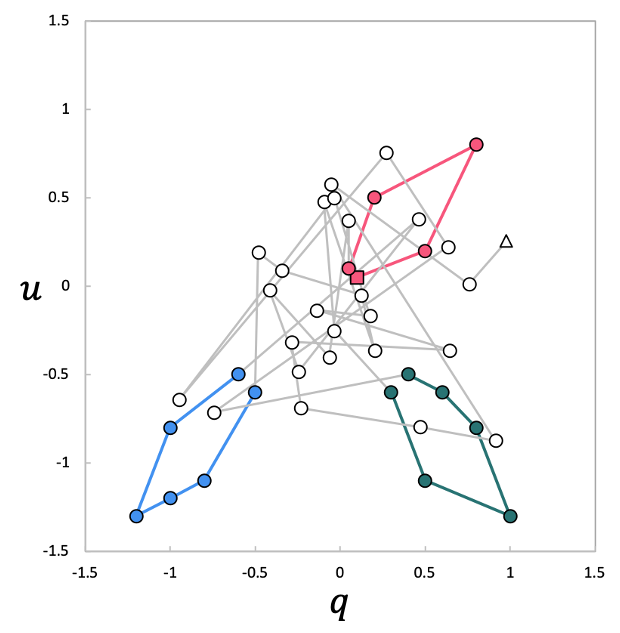
\includegraphics[width=.99\linewidth]{vgtc_journal_latex/figures/QBEdemodataStokes.png}
    % \end{minipage}
    % \begin{minipage}{0.44\linewidth}
    %     \centering
    %     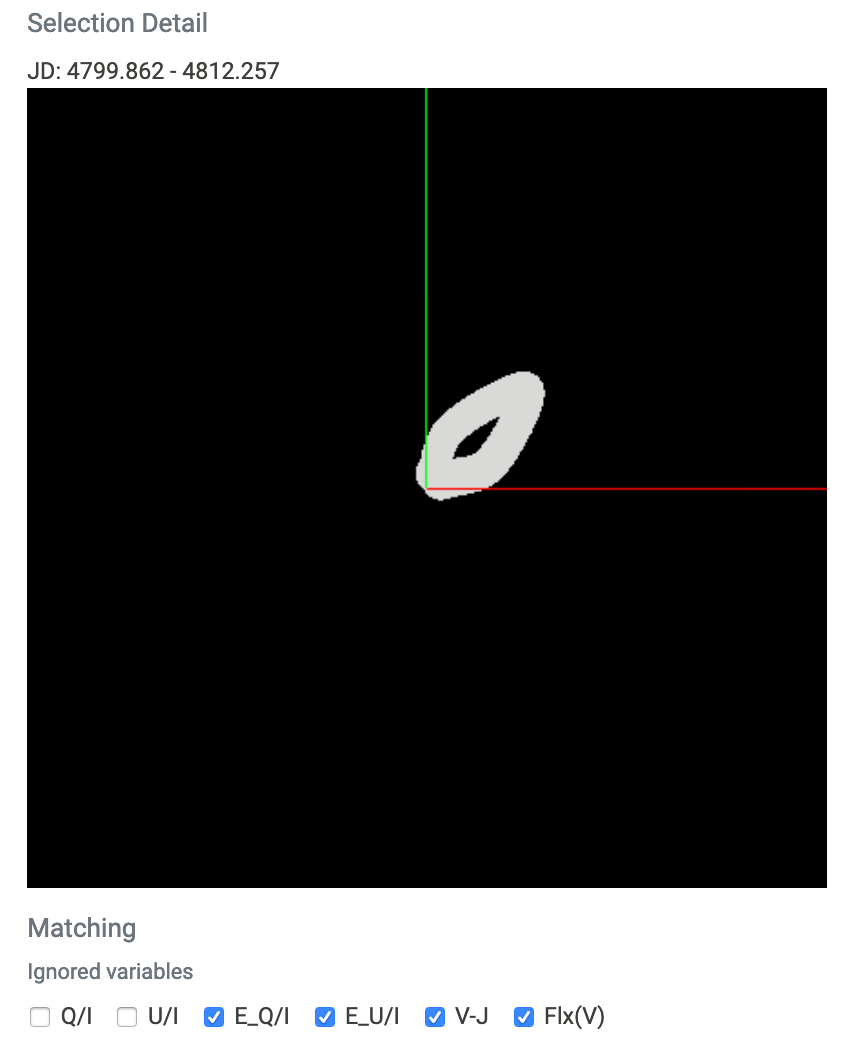
\includegraphics[width=.99\linewidth]{vgtc_journal_latex/figures/QBEdemodataQuery.png}
    % \end{minipage}\\
    % \begin{minipage}{0.55\linewidth}
    %     \centering
    %     \footnotesize{\sf (a)~The data on the Stoke plane.}
    % \end{minipage}
    % \begin{minipage}{0.44\linewidth}
    %     \centering
    %     \footnotesize{\sf (b)~Selected time interval.}
    % \end{minipage}\\
    
    % \footnotesize{\sf (c)~Results of QBE with the query in (a).}
    

% \begin{figure}[tb]
%     \centering
%     \includegraphics[width=.99\linewidth]{images/QBSMenuLabel.png}
%     \caption{Query specification in the query-by-sketch. (a)~Sketch pad. (b)~Filter constraint assignment. (c)~Parameter setting for the sketch.}
%     \label{fig:QBS}
% \end{figure}

% It is obvious that QBS supports \textbf{T5}. 


% DTW is a common algorithm for measuring similarity between two time series.
% Why dynamic time warping?

% When comparing two time-dependent, multi-dimensional data $Q$ and $C$ with $M$ dimensions, %whose length is $l_Q$ and $l_C$ respectively,
% the distance (${\rm DTW}_{\rm I} (Q, C)$) between two time series is expressed by the following equation:
% \begin{eqnarray}
% \label{equ:distanceDTWI}
%     {\rm DTW}_{\rm I} (Q, C) = \sum_{m = 1}^{M}{\rm DTW}(Q_m, C_m).
%     % d(q_{i, m}, c_{j, m}) = \sqrt{(q_{i, m} - c_{j, m})^2}
% \end{eqnarray}

% The following equation computes the distance (${\rm DTW}_{\rm D} (Q, C)$) between two time series $Q$ and $C$:
% \begin{eqnarray}
% \label{equ:distanceDTWD}
%     {\rm DTW}_{\rm D} (Q, C) = {\rm DTW}(\{Q_1, Q_2, \cdots, Q_M\}, \{C_1, C_2, \cdots, C_M\}).
%     % d(q_{i, m}, c_{j, m}) = \sqrt{(q_{i, m} - c_{j, m})^2}
% \end{eqnarray}

% The following part explains DTW for multi-dimensional data.
% Data $Q$ and $C$ is a collection of $M$ time series whose length is $l_Q$ and $l_C$ respectively:
% \begin{eqnarray*}
%     Q_1 &=& q_{1, 1}, q_{2, 1}, \cdots , q_{l_Q, 1} \\
%     Q_2 &=& q_{1, 2}, q_{2, 2}, \cdots , q_{l_Q, 2} \\
%     \cdots \\
%     Q_M &=& q_{1, M}, q_{2, M}, \cdots , q_{l_Q, M}
% \end{eqnarray*}
% \begin{eqnarray*}
%     C_1 &=& c_{1, 1}, c_{2, 1}, \cdots , c_{l_C, 1} \\
%     C_2 &=& c_{1, 2}, c_{2, 2}, \cdots , c_{l_C, 2} \\
%     \cdots \\
%     C_M &=& c_{1, M}, c_{2, M}, \cdots , c_{l_C, M}
% \end{eqnarray*}
% For ${\rm DTW}_{\rm I}$, we construct $M$ $l_Q-$by$-l_C$ distance matrix, where the $(i_m, j_m)$ element is the distance $d(q_{i, m}, c_{j, m})$ between two points $q_{i, m}$ and $c_{j, m}$.
% \begin{eqnarray}
% \label{equ:distanceDTWI}
%     d(q_{i, m}, c_{j, m}) = \sqrt{(q_{i, m} - c_{j, m})^2}
% \end{eqnarray}
% The definition of the cumulative distance $D(i, j)$ of ${\rm DTW}_{\rm I}$ is same as DTW for single-dimensional time series.
% \begin{eqnarray}
% \label{equ:DDTWI}
%     D_m(i, j) = d(q_{i, m}, c_{j, m}) 
%     + \min \left\{
%     \begin{array}{l}
%         D_m(i - 1, j - 1), \\
%         D_m(i - 1, j), \\
%         D_m(i, j - 1)
%     \end{array}
%     \right\}
% \end{eqnarray}
% The $(l_Q, l_C)$ element in the distance matrix represents the maximum distance between $Q$ and $C$.
% In the case of ${\rm DTW}_{\rm I}$, therefore, the distance between two data $DTW_I$ is as follows:
% \begin{eqnarray}
% \label{eqn:DTWI}
%     DTW_I = \sum_{m=1}^{M} D_m(l_Q, l_C).
% \end{eqnarray}

% For ${\rm DTW}_{\rm D}$, we construct a $l_Q-$by$-l_C$ distance matrix, where the $(i_m, j_m)$ element is as follows:
% \begin{eqnarray}
% \label{eqn:distanceDTWD}
%     d(q_i, c_j) = \sum_{m = 1}^{M} \sqrt{(q_{i, m} - c_{j, m})^2}.
% \end{eqnarray}
% The cumulative distance $D(i, j)$ depends on the sum of distances computed in Equation \ref{eqn:distanceDTWD}.
% \begin{eqnarray}
% \label{equ:DDTWD}
%     D(i, j) = d(q_{i}, c_{j}) 
%     + \min \left\{
%     \begin{array}{l}
%         D(i - 1, j - 1), \\
%         D(i - 1, j), \\
%         D(i, j - 1)
%     \end{array}
%     \right\}
% \end{eqnarray}
% Finally, the maximum distance between two data $DTW_D$ is as follows:
% \begin{eqnarray}
% \label{eqn:DTWD}
%     DTW_D = D(l_Q, l_C).
% \end{eqnarray}

% \begin{figure}[tb]
%     \centering
%     \includegraphics[width=.99\linewidth]{images/ResultQuerying.png}
%     \caption{Users are allowed to re-utilize a result as a key for query-by-sketch.}
%     \label{fig:resultQuerying}
% \end{figure}

% By normalizing the query or using polar coordinates in the matching process, 
% our system can identify time intervals with similar shapes but different scales or those transformed, too.

% It is a chief card for \textbf{T4}.